%------------------------------------------------------------------------
% Chapter:  Using the mouse
%------------------------------------------------------------------------

\chapter{Using the mouse \label{mouse}}

%------------------------------------------------------------------------
\section{Mouse interface \label{mouse-interface}}

To enter the mouse mode, simply use the command {\tt mouse}. The
plot window will now contain a number off buttons in addition to the
view graph as can be seen in Figure \ref{mou-fig1}.
%
\begin{figure}[!b]
   \centering
   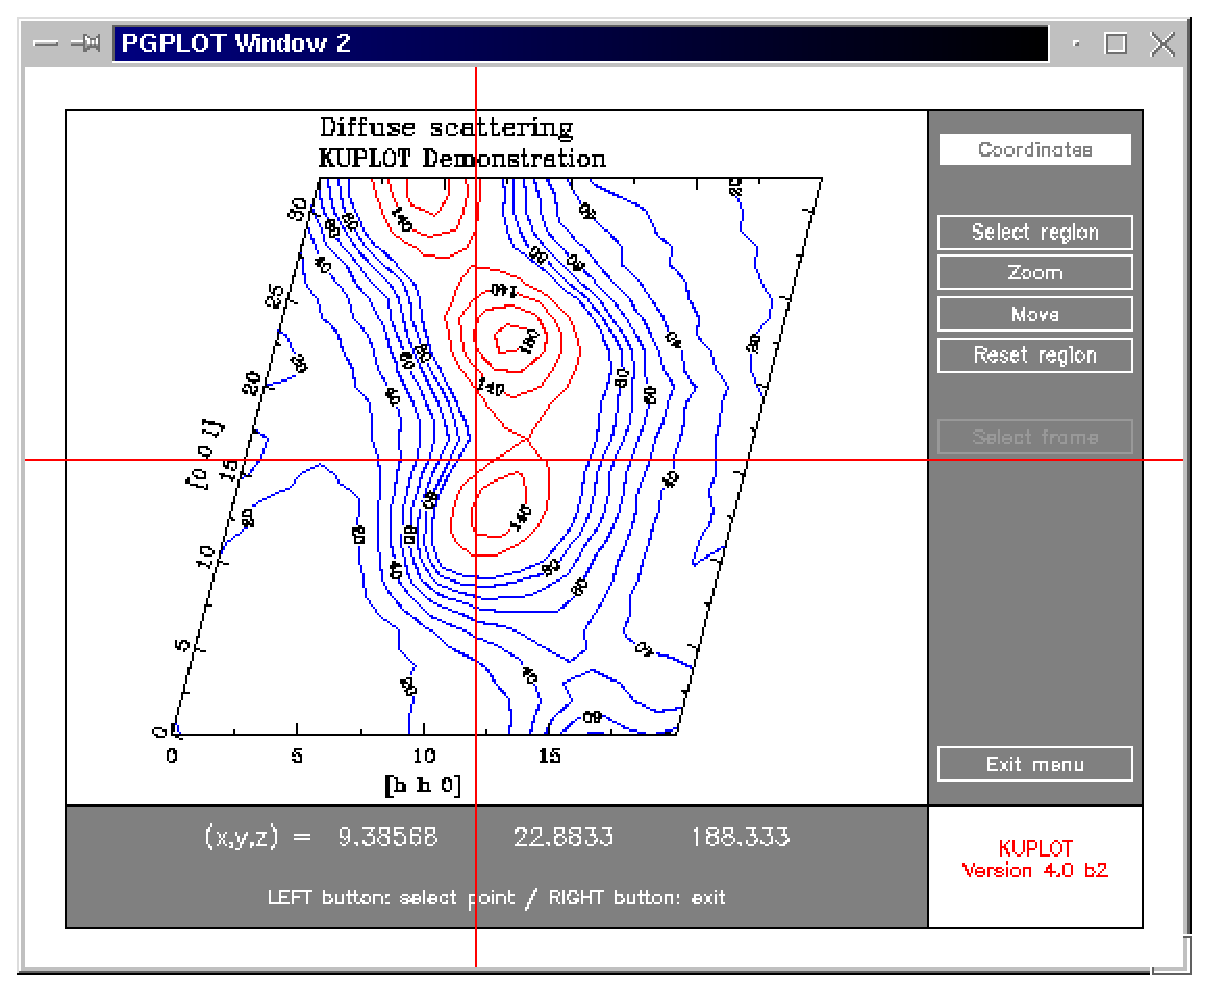
\includegraphics[scale=0.5]{mou.1.eps}
   \caption{{\it KUPLOT} in {\it mouse} mode}
   \label{mou-fig1}
\end{figure}
%
The button {\it Coordinates} allows the user to display the
coordinates of the mouse pointer by clicking the left mouse button.
The values are displayed below the plot. In case of 2D files, the
$z$-value of the closest data point is also shown. The right mouse
button terminates the coordinate display function. The next group of
buttons allows the user to use the mouse to modify the potting area.
{\it Select region} does exactly that by clicking on the lower left
corner of the desired area first. A moving frame will appear and the
user can select the other corner of the new region. The buttons {\it
Zoom} and {it Move} perform these functions using all three mouse
buttons. A short help text explaining which button is doing what
appears below the plotting area once a function is selected. 'Reset
region' allows the user to quickly display the complete range of
data again. In cases where the current plot contains frames (see
chapter \ref{frame}), the active frame is marked by a light red
background color. All functions will affect the active frame only.
The focus can be moved to another frame via the {\it Select frame}
button, which is only active when there is more than a single frame.
Finally to get back to the command prompt of {\it KUPLOT} use the
{\it Exit menu} button. Note that in cases where commands are
written to a macro file via the command {\tt learn}, all region
functions will write the corresponding {\tt skal} command in the
macro file. One should also be careful when using the {\tt mouse}
command in macro files, since {\it KUPLOT} will not execute any
further commands in until the {\it Exit menu} button is hit.
\par

%------------------------------------------------------------------------
\section{Mouse in macros \label{mouse-mac}}

In the previous section, we learned about the interactive interface
of {\it KUPLOT}. Alternatively, the {\tt mouse} command can have
additional parameters which specify what will be selected using the
mouse pointer. In this case no buttons will show up and the
coordinates will be returned in the {\tt res[]} variables. Let us
consider the following example. The goal is to use the mouse to
select a number of points and store those in a data set. This could
e.g. be used to define a background underneath some data manually.
The macro file is show here:
%
\begin{MacVerbatim}
    1  variable integer,pt
    2  variable integer,npt
    3  variable integer,button
    4  #
    5  npt=0
    6  button=0
    7  #
    8  echo Select points - right mouse button to finish
    9  #
   10  do while (button.ne.3)
   11    mouse point
   12    npt=npt+1
   13    r[100+npt]=res[1]
   14    r[200+npt]=res[2]
   15    button=res[3]
   16  enddo
   17  #
   18  npt=npt-1
   19  alloc back,npt
   20  do pt=1,npt
   21    x[n[1],pt]=r[100+pt]
   22    y[n[1],pt]=r[200+pt]
   23  enddo
   24  #
   25  plot
\end{MacVerbatim}
%
We assume the data set of interest has been loaded and one has
zoomed into the area where the background should be defined. In
lines 1--3 we define the required variables. Note that this uses the
new feature of named variables discussed in more detail in the chapter
{\tt Fortran style interpreter} of the general package manual
\href{./package\_man.pdf}{DISCUS package}. In lines 5 and 6 some variables are initially set to
zero. In line 8 a message is printed on the screen to tell the user
what to do. Basically every left click with the mouse will define a
point and a right click will exit the macro and store the selected
points. In line 10 we start a {\tt while} loop which is executed
until the variable {\tt button} contains the number 3 which
corresponds to the clicking the right mouse button. The command {\tt
mouse point} allows the user to select a point. The coordinates and
the button pressed are returned in variables {\tt res[i]} and are
stored in variables (lines 13--15). This loop is now repeated until
the right mouse button is pressed. Every time the variable {\tt npt}
is incremented, containing the number of points selected so far. The
way the loop is constructed, {\tt npt} actually contains the number
of points plus on which is fixed in line 18. The command {\tt alloc}
(line 19) now creates a new and empty {\it KUPLOT data set} with a
size of {\tt npt} points. The loop in lines 20--23 is then used to
store the coordinates selected in that data set and finally the data
and background data set are plotted (line 25). In reality one would
add commands to either interpolate and subtract the background
directly or store it in a data file. The command {\tt mouse} can
also be used to select a region or range (see Table \ref{mou-tab1}).

%
\begin{table}[!t]
\centering
\begin{tabularx}{\textwidth}{|p{15mm}|X|}
  \hline
  {\bf Mode} & {\bf Description} \\
  \hline\hline
  point   & Selects a single point and returns $x,y$ or $x,y,z$ in
            variable {\tt res[i]}.\\
  line    & Selects two points connected by a line.\\
  rect    & Selects two corners of a rectangle.\\
  xrange  & Selects two points defining range in $x$.\\
  yrange  & Selects two points defining range in $y$.\\
  \hline
\end{tabularx}
\caption{\label{mou-tab1}Modes of command {\tt mouse}}
\end{table}
%

%------------------------------------------------------------------------
